\documentclass[12pt, twoside]{article}
\documentclass[12pt, twoside]{article}
\usepackage[letterpaper, margin=1in, headsep=0.2in]{geometry}
\setlength{\headheight}{0.6in}
%\usepackage[english]{babel}
\usepackage[utf8]{inputenc}
\usepackage{microtype}
\usepackage{amsmath}
\usepackage{amssymb}
%\usepackage{amsfonts}
\usepackage{siunitx} %units in math. eg 20\milli\meter
\usepackage{yhmath} % for arcs, overparenth command
\usepackage{tikz} %graphics
\usetikzlibrary{quotes, angles}
\usepackage{graphicx} %consider setting \graphicspath{{images/}}
\usepackage{parskip} %no paragraph indent
\usepackage{enumitem}
\usepackage{multicol}
\usepackage{venndiagram}

\usepackage{fancyhdr}
\pagestyle{fancy}
\fancyhf{}
\renewcommand{\headrulewidth}{0pt} % disable the underline of the header
\raggedbottom
\hfuzz=2mm %suppresses overfull box warnings

\usepackage{hyperref}
\usepackage{float}

\title{Algebra 2}
\author{Chris Huson}
\date{June 2024}

\fancyhead[LE]{\thepage}
\fancyhead[RO]{\thepage \\ Name: \hspace{1.5cm} \,\\}
\fancyhead[LO]{BECA/Huson/Algebra 2: Regents Preparation \\* 6 June 2024}

\begin{document}
\subsubsection*{Prep \#24 Exponential regression}
Casio instructions: \url{https://www.youtube.com/watch?v=jcX93Grn8o8} \\[0.25cm]
Menu \textgreater{} Stat \textgreater{} enter data in List 1 and List 2 \\ \textgreater{} Calc (F2) \textgreater{} REG (F3) \textgreater{} (F6) \textgreater{} EXP (F2) \textgreater{} ab\textasciicircum{}X (F2)
\begin{enumerate}[itemsep=0.5cm]
\item Consider the data in the table below.
    \begin{center}
    \begin{tabular}{|p{1cm}|p{1cm}|p{1cm}|p{1cm}|p{1cm}|p{1cm}|p{1cm}|}
        \hline
        $x$ & 1 & 2 & 3 & 4 & 5 & 6 \\
        \hline
        $y$ & 3.9 & 6 & 11 & 18.1 & 28 & 40.3 \\[0.25cm]
        \hline
    \end{tabular}
    \end{center}
    State an exponential regression equation to model these data, rounding all values to the \emph{nearest thousandth}.  \vspace{2cm} %Regents Jan2023
    % y = 2.459(1.616)^x

\item A cup of coffee is left out on a countertop to cool. The table below represents the temperature, $F(t)$, in degrees Fahrenheit, of the coffee after it is left out for $t$ minutes.
    \begin{center}
    \begin{tabular}{|p{1cm}|p{1cm}|p{1cm}|p{1cm}|p{1cm}|p{1cm}|p{1cm}|}
        \hline
        $t$ & 0 & 5 & 10 & 15 & 20 & 25 \\
        \hline
        $F(t)$ & 180 & 144 & 120 & 104 & 93.3 & 86.2 \\[0.25cm]
        \hline
    \end{tabular}
    \end{center}
    Based on these data, write an exponential regression equation, $F(t)$, to model the temperature of the coffee. Round all values to the \emph{nearest thousandth}.  \vspace{2cm} %Regents Jun2022
    % F(t) = 169.136 (0.971)^t

\item Kelly-Ann has \$20,000 to invest. She puts half of the money into an account that grows at an annual rate of 0.9\%. %compounded monthly
At the same time, she puts the other half of the money into an account that grows continuously at an annual rate of 0.8\%. Write an equation that represents the value of Kelly-Ann's investments after $t$ years.
    
\newpage
\item An investment of \$5000 grows at an annual rate of 3.5\% compounded monthly. 
$$P(t)=5000(1+\frac{0.035}{12})^{12t}$$
\begin{enumerate}
    \item Find the investment value after 10 years. \vspace{2cm}
    \item Determine the time for the investment value to double, to the \emph{nearest month}. \vspace{3cm}
\end{enumerate}

\item The table below gives air pressures in kPa at selected altitudes above sea level measured in kilometers.
\begin{center}
    \begin{tabular}{|p{1cm}|p{4cm}|p{1cm}|p{1cm}|p{1cm}|p{1cm}|p{1cm}|p{1cm}|}
        \hline
        $x$ & Altitude (km) & 0 & 1 & 2 & 3 & 4 & 5 \\
        \hline
        $y$ & Air Pressure (kPa) & 101 & 90 & 79 & 70 & 62 & 54 \\[0.25cm]
        \hline
    \end{tabular}
    \end{center}
    Write an exponential regression equation that models these data rounding all values to the \emph{nearest thousandth}. \\[2cm]
    Use this equation to algebraically determine the altitude, to the \emph{nearest hundredth} of a kilometer, when the air pressure is 29 kPa. %Regents Jan2020

\newpage
\item Expand and simplify each complex expression.
\begin{multicols}{2}
\begin{enumerate}
    \item $6xi^3(-4xi+5)$
    \item $(x+3i)^2-(2x-3i)^2$
\end{enumerate}
\end{multicols} \vspace{4cm}

\item Solve each equation. Express the answer in $a+bi$ form.
\begin{multicols}{2}
\begin{enumerate}[itemsep=0.5cm]
    \item $2x^2+5x+8=0$
    \item $5x^2-2x+13=9$ %Regents Aug2019
\end{enumerate}
\end{multicols} \vspace{4cm}

\item Find the solution set of each equation (round to the \emph{nearest tenth}).
\begin{multicols}{2}
    \begin{enumerate}
        \item $\displaystyle \frac{2}{3x+1} = \frac{1}{x} - \frac{6x}{3x+1}$
        \item $\displaystyle \frac{1}{1-x^2} = - |3x-2|+5$
    \end{enumerate}
\end{multicols}

\newpage
\item Over the set of integers, factor completely $x^4-5x^2+4$. \vspace{3cm} %Regents Jan2023

\item Determine which expressions are equivalent to $\displaystyle \frac{x^4-5x^2+4x+14}{x+2}$. \\[0.25cm]
    (hint: substitute $x=0$ and $x=1$)
    \begin{multicols}{2}
    \begin{enumerate}[itemsep=2cm]
        \item $\displaystyle x^3-2x^2-x+6+\frac{2}{x+2}$
        \item $\displaystyle x^3-5x+4-\frac{14}{x+2}$
        \item $\displaystyle x^3+2x^2-x+2+\frac{18}{x+2}$
        \item $\displaystyle x^3+2x^2-9x+22-\frac{30}{x+2}$
    \end{enumerate}
    \end{multicols} \vspace{2cm}

\item Given $a > 0$, solve the equation $a^{x+1} = \sqrt[3]{a^2}$ for $x$ algebraically. %Regents Jan2023
\vspace{2cm}

\newpage
\subsubsection*{Prep \#24 Periodic functions}
\item The function $f(x)= \sin x$ is shown on the graph below. 
\begin{center}
    \begin{tikzpicture}[xscale=2]
        \draw[gray,thin] (0,-3) grid[xstep=pi/8] (6.3,3);
        \draw [thick,->] (0,0)--(6.5,0) node [right] {$x$};
        \draw [thick,->] (0,-3)--(0,3.5) node [right] {$y$};
        \foreach \x/\xtext in {0.5*pi/$\frac{1}{2}\pi$, pi/$\pi$, 1.5*pi/$\frac{3}{2}\pi$,2*pi/$2\pi$}
            \draw (\x,5pt) -- (\x,-5pt) node[below] {\xtext};
        \foreach \y in {-3,...,3}
            \draw (2pt,\y cm)--(-2pt,\y cm) node[left]{$\y$};
        \draw [thick,->, domain=0:2*pi+0.25,smooth,samples=100] plot (\x,{sin(\x r)});
    \end{tikzpicture}
    \end{center}
    \begin{enumerate}
        \item A second periodic function $g(x)$ has an amplitude of 2. Graph $g(x)=2\sin x$ on the same set of axes as $f(x)$.
        \item Find $g(\frac{3}{4}\pi)$ as an exact value. Mark the point on the graph and label it as an ordered pair.
    \end{enumerate}

\item Graph the function $f(x)= 3 \sin x +5$. Draw and label the midline of $f$, $y=5$.
\begin{center}
    \begin{tikzpicture}[xscale=2, yscale=0.8]
        \draw[gray,thin] (0,0) grid[xstep=pi/8] (6.3,9);
        \draw [thick,->] (0,0)--(6.5,0) node [right] {$x$};
        \draw [thick,->] (0,0)--(0,9.5) node [right] {$y$};
        \foreach \x/\xtext in {0.5*pi/$\frac{1}{2}\pi$, pi/$\pi$, 1.5*pi/$\frac{3}{2}\pi$,2*pi/$2\pi$}
            \draw (\x,5pt) -- (\x,-5pt) node[below] {\xtext};
        \foreach \y in {0,...,9}
            \draw (2pt,\y cm)--(-2pt,\y cm) node[left]{$\y$};
    \end{tikzpicture}
    \end{center}

\newpage
\item A periodic function $f(x)$ is shown on the graph below.
\begin{enumerate}
    \item Draw and label as an equation the midline of $f$.
    \item Mark the maximum and minimum points of $f$ over the graphed domain, and label them as ordered pairs.
    \item Write down an equation for the function in the form $f(x)=A \sin x+D$. \vspace{2cm}

\begin{center}
    \begin{tikzpicture}[xscale=2, yscale=0.4]
        \draw[gray,thin] (0,0) grid[xstep=pi/8,ystep=2] (6.3,20);
        \draw [thick,->] (0,0)--(6.5,0) node [right] {$x$};
        \draw [thick,->] (0,0)--(0,20.5) node [above] {$f(x)$};
        \foreach \x/\xtext in {0.5*pi/$\frac{1}{2}\pi$, pi/$\pi$, 1.5*pi/$\frac{3}{2}\pi$,2*pi/$2\pi$}
            \draw (\x,5pt) -- (\x,-5pt) node[below] {\xtext};
        \foreach \y in {0,2,...,20}
            \draw (2pt,\y cm)--(-2pt,\y cm) node[left]{$\y$};
        \draw [thick,->, domain=0:2*pi+0.25,smooth,samples=100] plot (\x,{6*sin(\x r)+10});
        \fill (2,{6*sin(2 r)+10}) ellipse (1pt and 5pt);
        \fill (3,{6*sin(3 r)+10}) ellipse (1pt and 5pt);
        \end{tikzpicture}
    \end{center}
    \item Find the average rate of change of $f(x)$ over the interval $2 < x < 3$ rounded to the \emph{nearest hundredth}.
\end{enumerate}


\end{enumerate}
\end{document}